\chapter{Simulation Methods}

\section{Introduction}
In a flow where an interface exists there is a need for interface reconstruction. \cite{Hirt1981} came up with the idea of Volume of Fluid interface{(VOF)} tracking to approximate
the free boundaries in numerical simulations. This method is based on a concept of fractional volume of fluid. This is still widely used due to its flexibility and efficiency
compared to other methods.
Volume of fluid essentially conserves the mass, where in level set method is better in reconstruction of curved interfaces.

\section{The Volume of Fluid method}
This method starts with defining a quantity called as volume fraction F, for each cell in computational domain. For a binary phase system there is a dark fluid and light fluid.
F is the ratio of volume of the dark fluid to the volume of the cell itself. The cells with only light fluid will have F = 0 and for only dark fluid F = 1. For interfacial cells
F will have a value between 0 and 1. The volume of fluid when advected it does not change with respect to the fluid parcel. Hence, it satisfies the following relation,
\begin{equation}
 \frac{\partial F}{\partial t}+(\overrightarrow u. \overrightarrow \nabla)F=0
\end{equation}
Now, F can be tracked in time using finite difference technique and use some algorithms to reconstruct the interface. But this methodolgy goes into problems as the smearing of interface,
due to the fact that F is a discontinuos fuction in spacial and temporal domain. There is need for some other technique to evolve interface in time. Here comes the role of geometrical reconstruction
and tracking of F-field. There are many such algorithms developed to demonstrate this such as SLIC, PLIC, Youngs method, LVIRA, ELVIRA etc.

\section{Motivation for a new method}
A need of new method arises when conventional methods fail. For multiphase flow, we can try to advect a material property say volume fraction of a fluid in the cell in time,
which follows the Eq 1.1.If we use finite difference method to solve above equation to advect the volume fraction, the interface does not remain sharp, smears, due to the fact that the volume
fractio is a step function but finite differencing tries to smooth it over the time. The conventional numerical methods do not retain the discontinuos property of the function. Hence there is need for methods 
which conserve the discontinuos material properties in multiphase flows.
\begin{figure}[tbp]
\raggedright
\begin{tabular}{p{7cm}p{5cm}}
\subfloat[Ini]{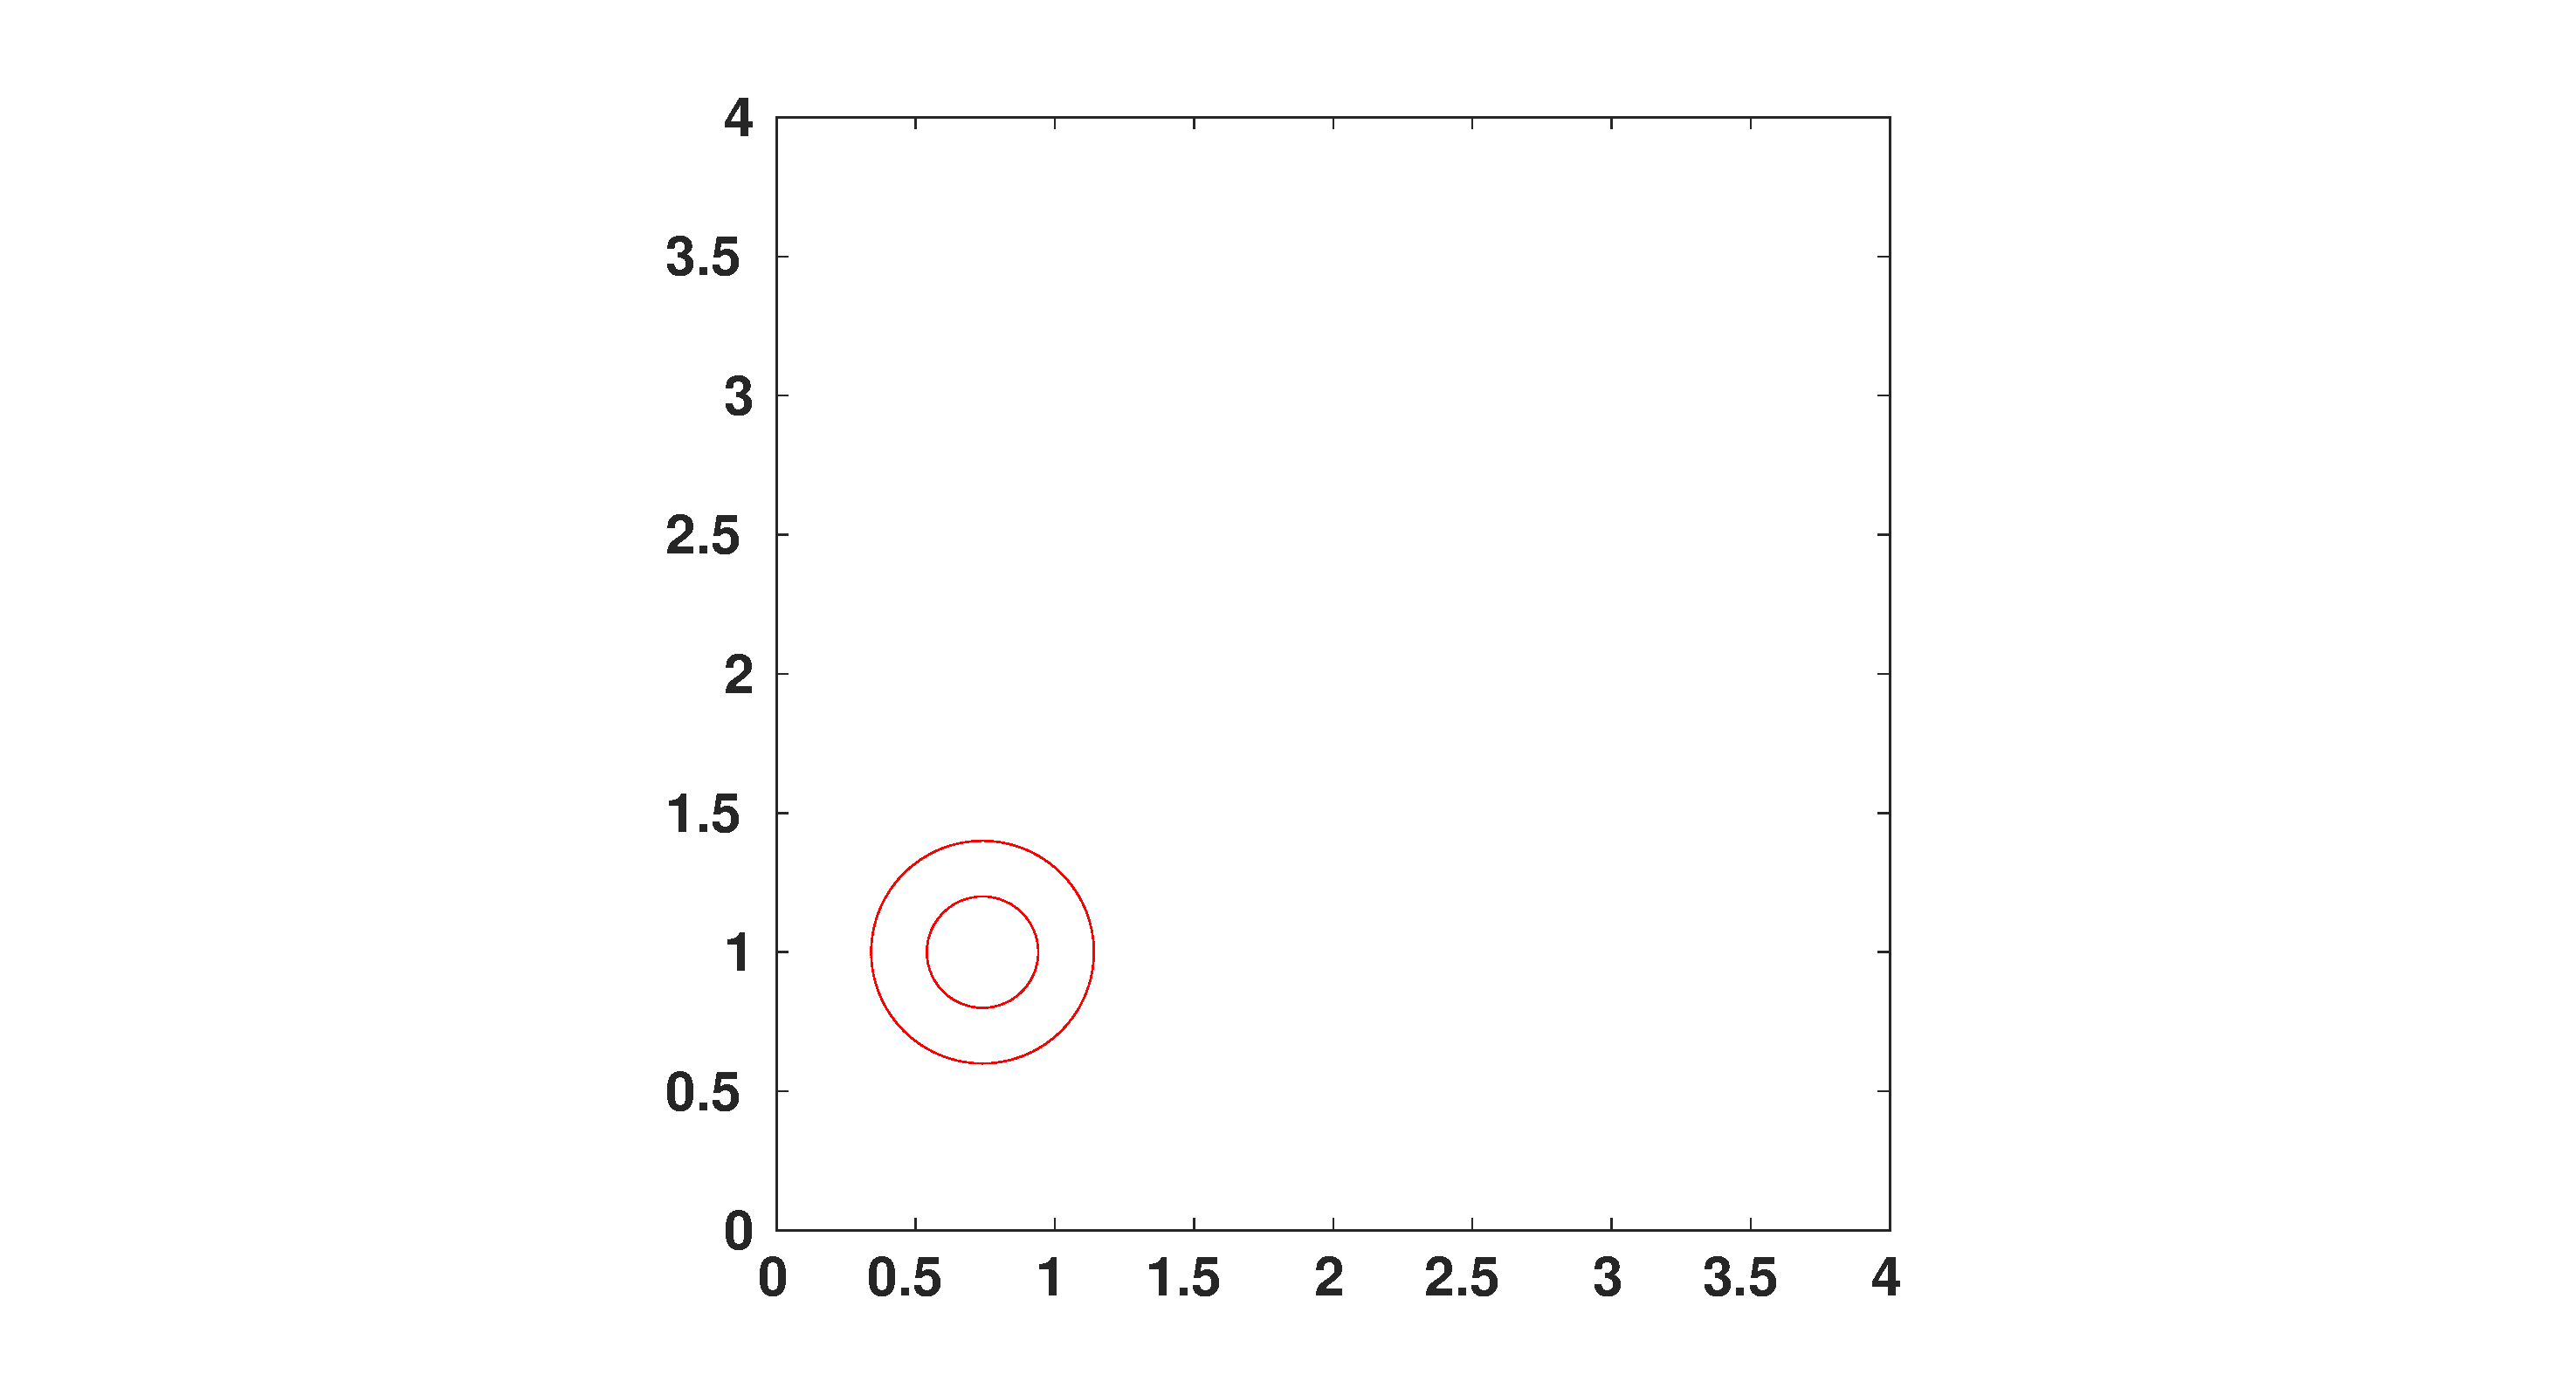
\includegraphics[scale=0.2]{CD_0.eps}} 
   & \subfloat[After advecs]{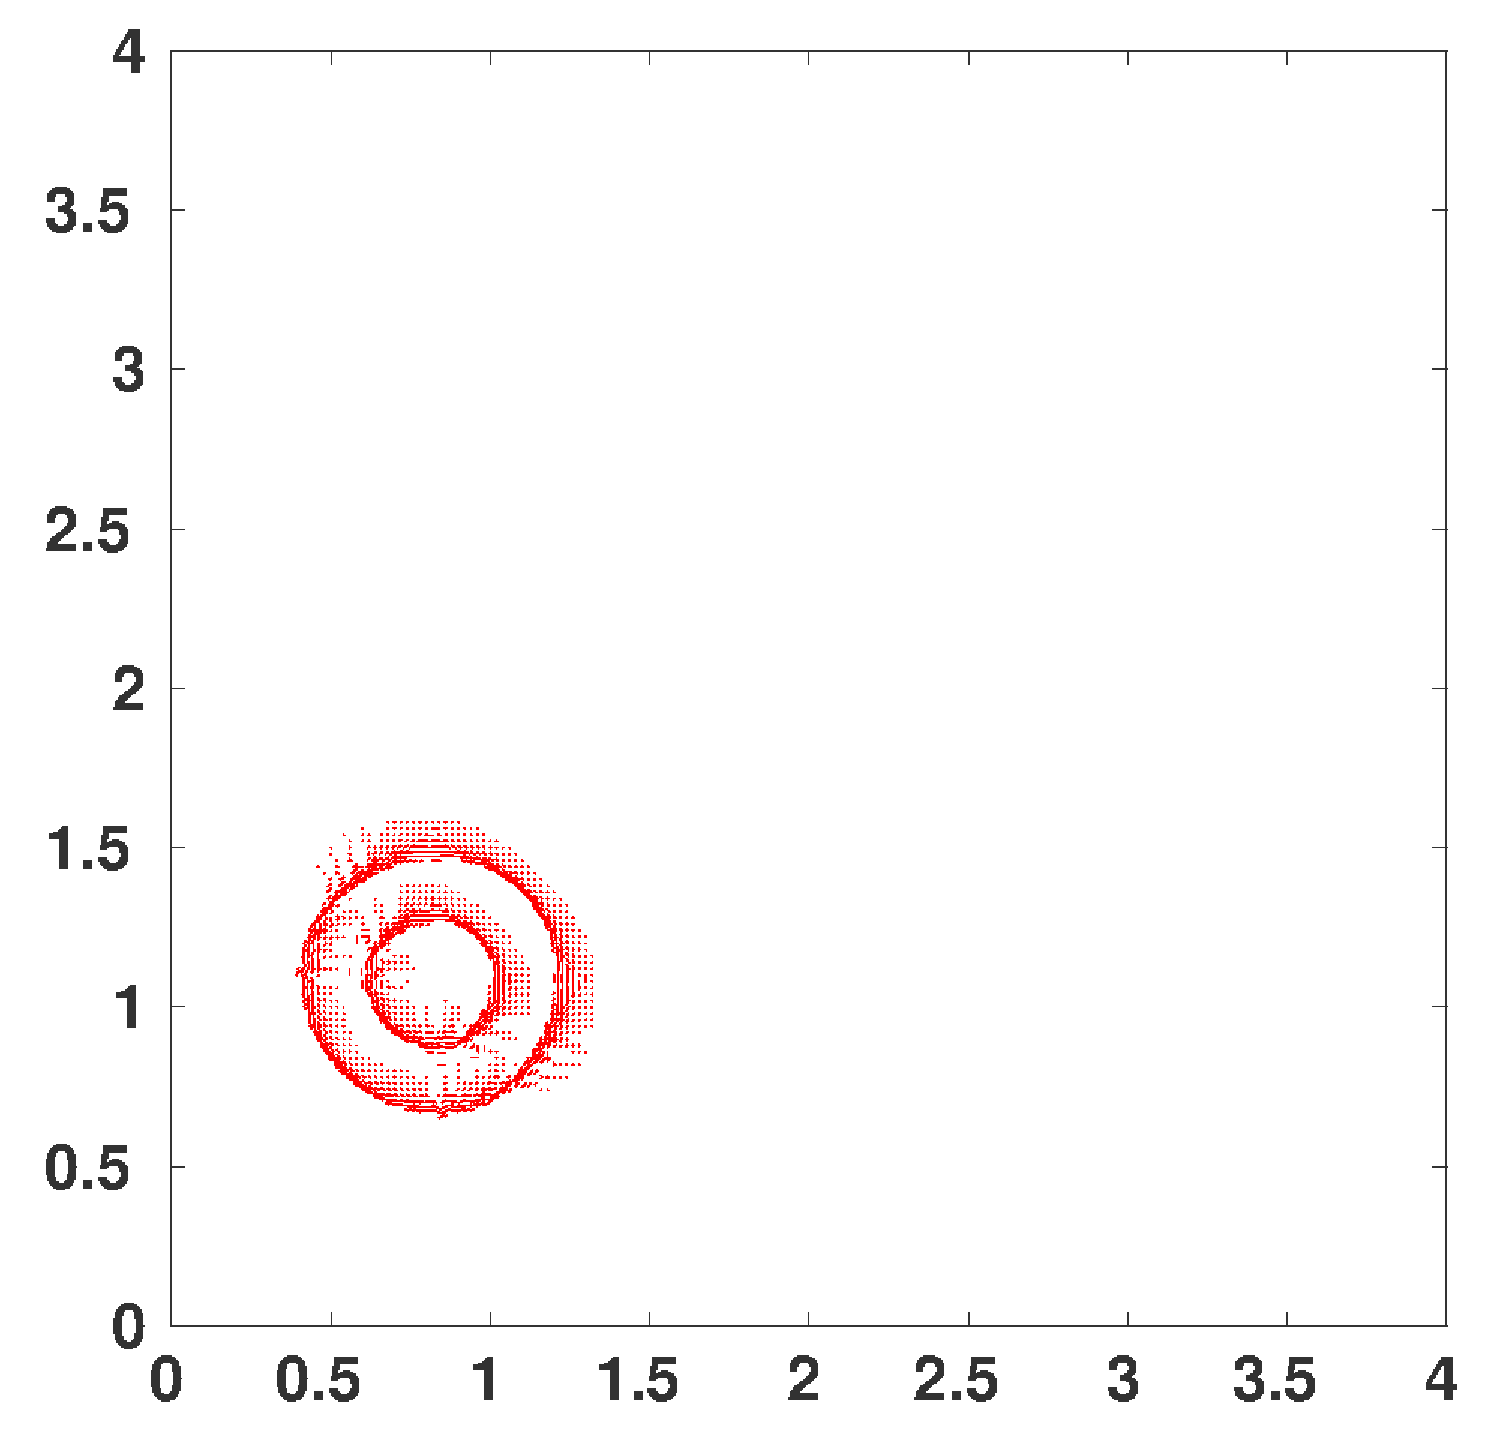
\includegraphics[scale=0.2]{CD_20.eps}}\\
\subfloat[After adve]{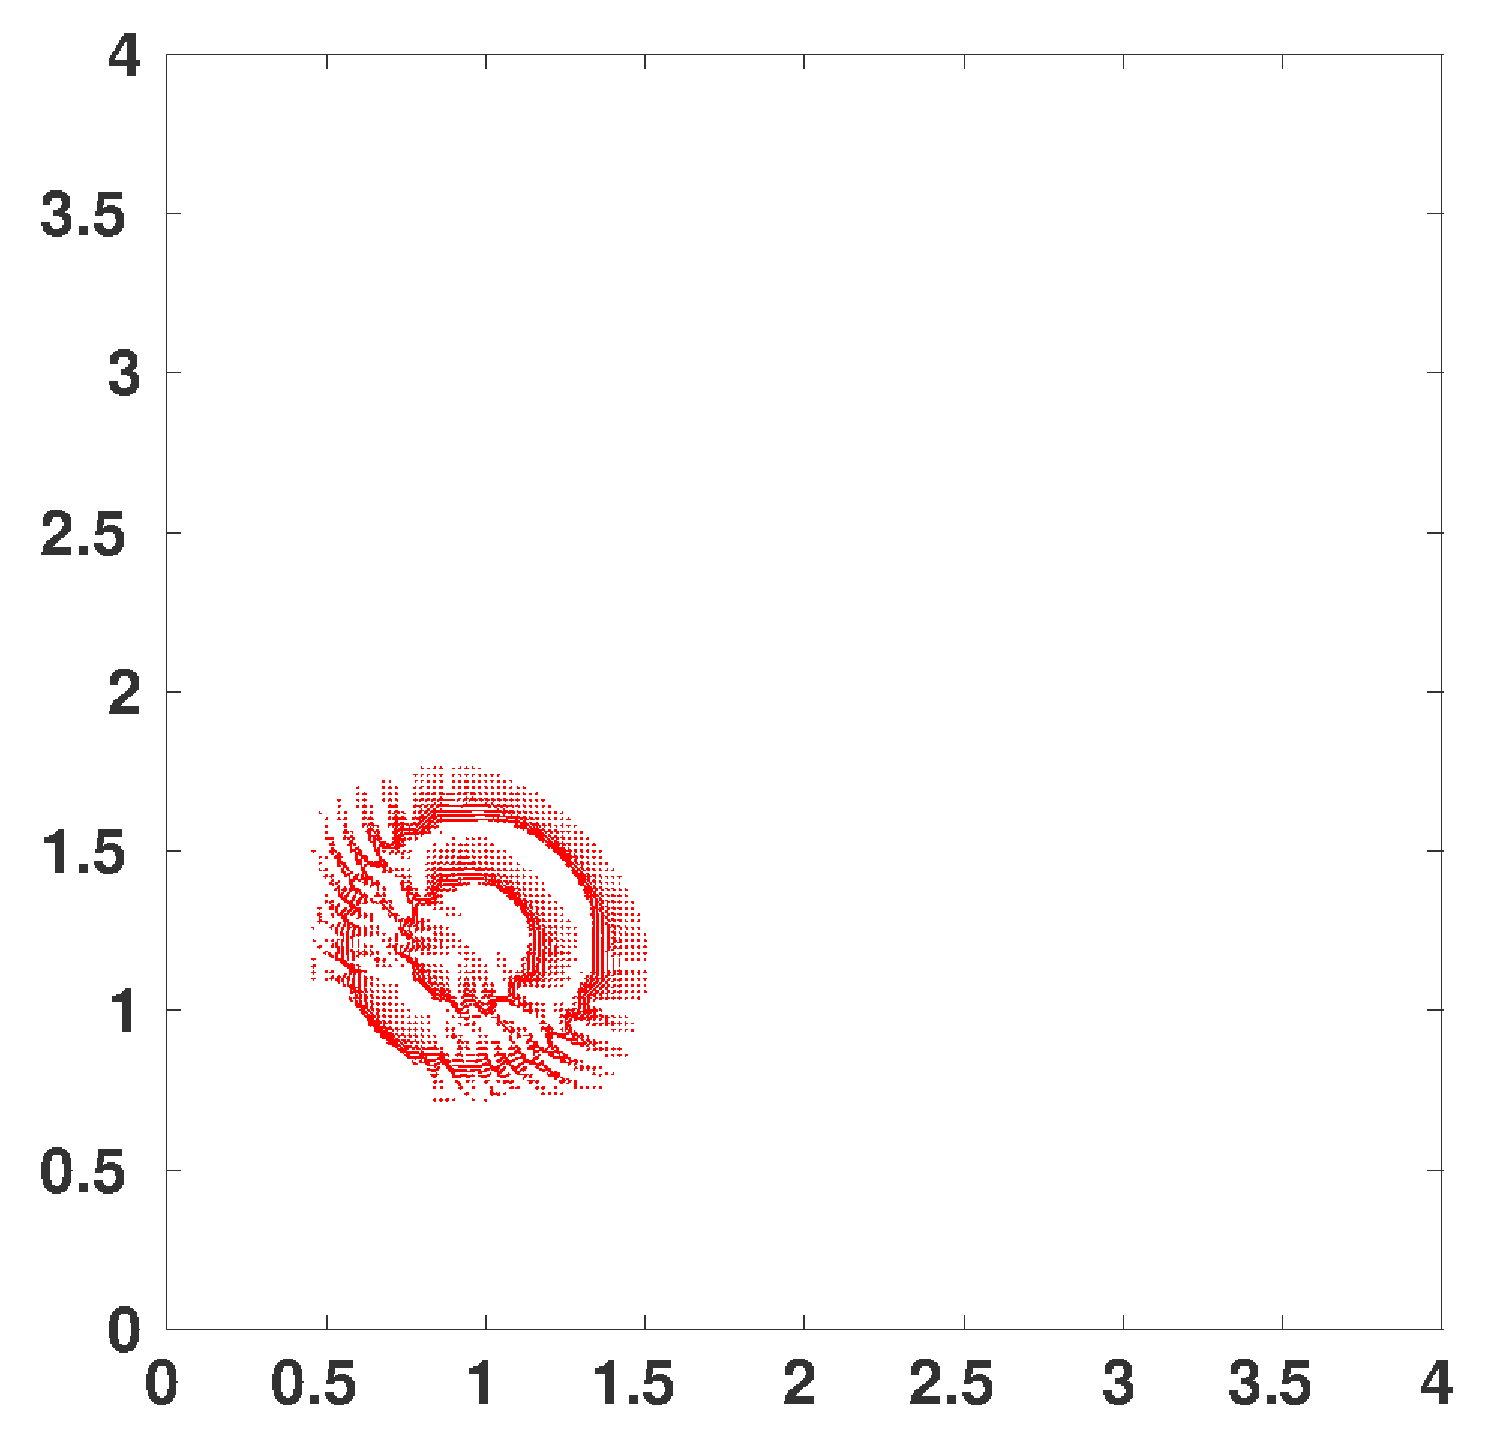
\includegraphics[scale=0.2]{CD_50.eps}} 
   & \subfloat[After ads]{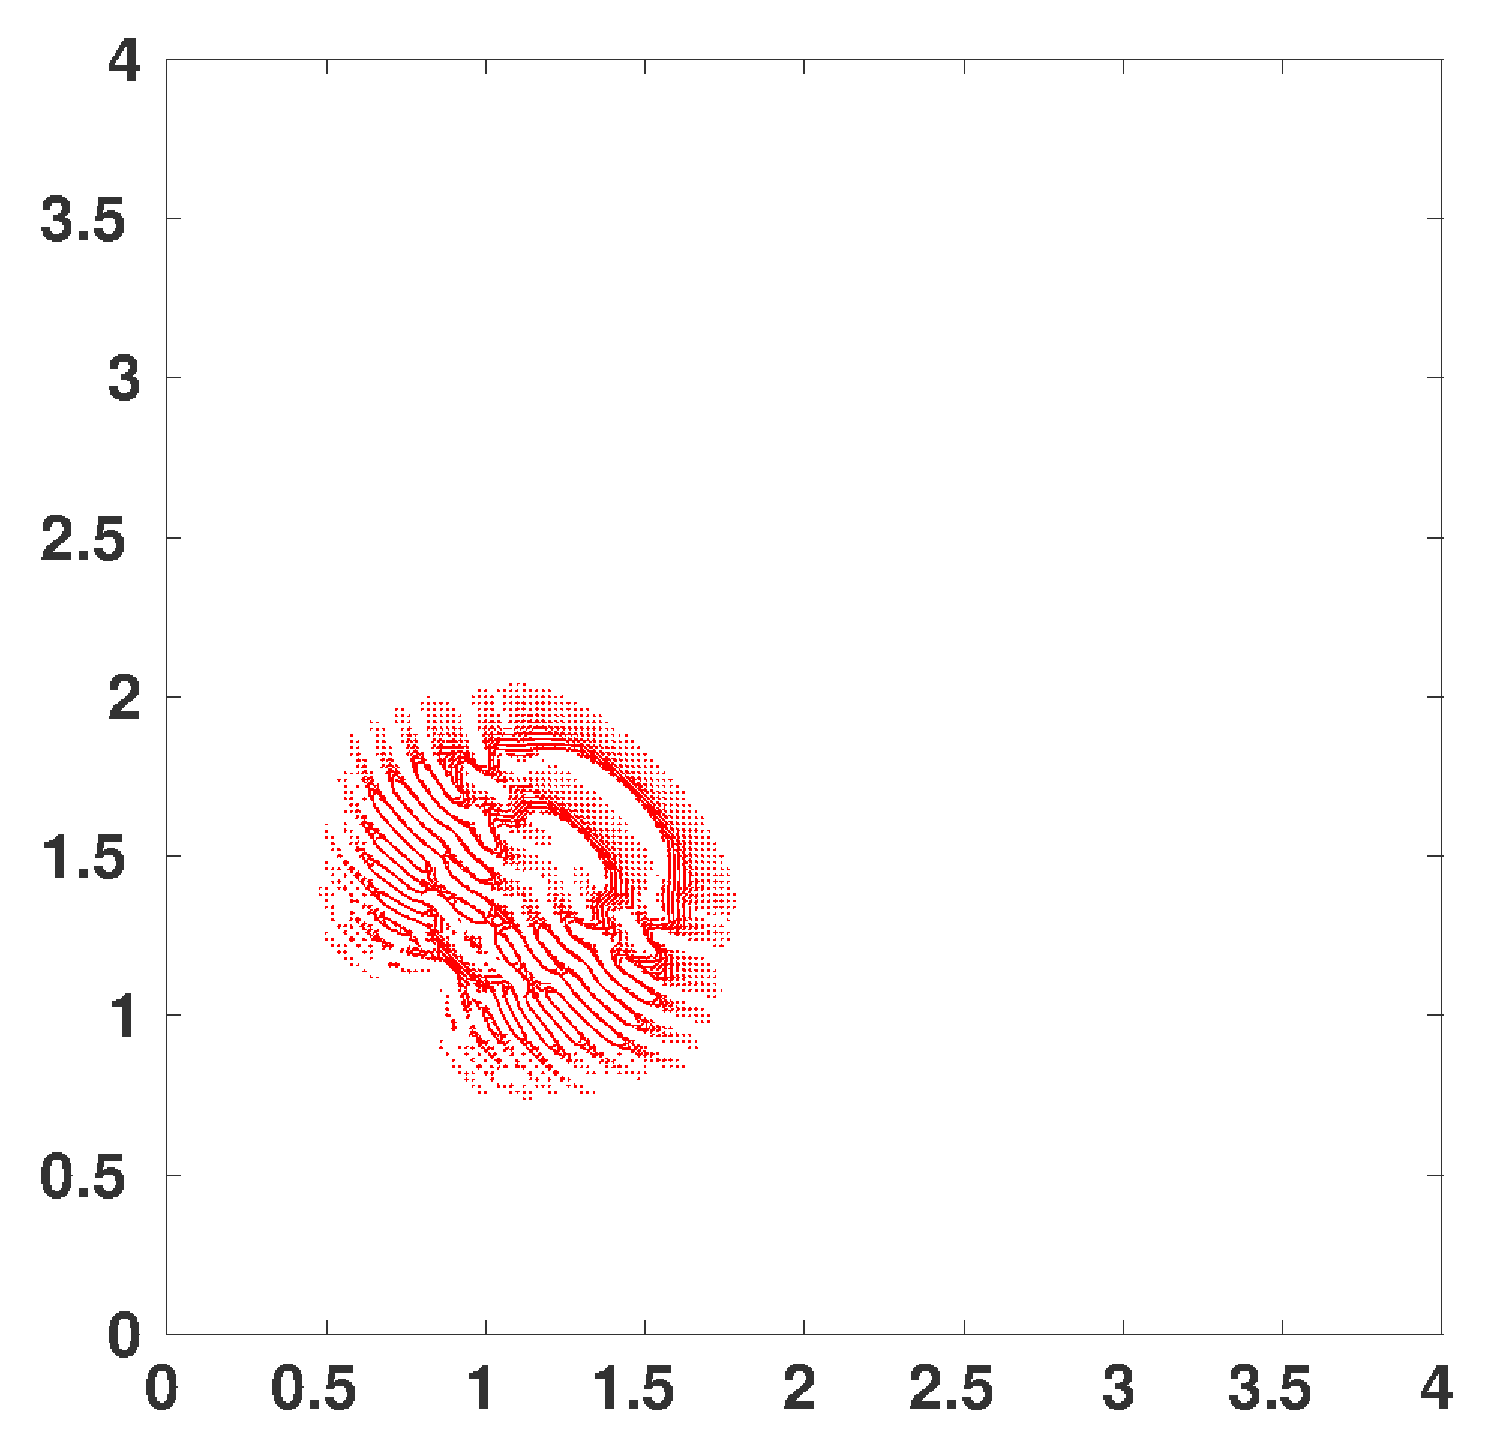
\includegraphics[scale=0.2]{CD_100.eps}}\\  
\end{tabular}
\caption{Advecting volume fraction using finite difference method}\label{figure1}
\end{figure}

\section{Least Squares of Volume of Fluid Interface Reconstruction Algorithm}
The interfaces in Volume of fluid method has no unique way of reconstruction. With a given F-field there are multiple algorithms to represent interface. One such algorithm is Least Squares Volume of 
Fluid Reconstruction Algorithm proposed by \cite{Pilliod2004}. It represents interface as a line in 2D and a plane in 3D.
Any interface reconstruction algorithm consists two basic steps:-
\begin{enumerate}
 \item Interface Reconstruction
 \item Advection of F field
\end{enumerate}

\section{Interface Reconstruction}
There are many steps involved in interface reconstruction explained in subsections.

\subsection{Step I : Obtain F field}
At first a F-field is obtained by knowing the initial free surface and then by calculating the F values in each cell. Then locate a cell having a value of F betwenn 0 and 1.

\subsection{Step II : Initial guess of slope}
The initial slope of the normal to the interface away from the dark fluid can obtained using Green-Guass gradient given by 
\begin{eqnarray}
  N_x=-\frac{1}{\Delta x}{[F_{r+1,c+1}+2F_{r,c+1}+F_{r-1,c+1}-F_{r+1,c-1}-2F_{r,c-1}-F_{r-1,c-1}]} \\
  N_y=-\frac{1}{\Delta y}{[F_{r+1,c+1}+2F_{r+1,c}+F_{r+1,c-1}-F_{r-1,c+1}-2F_{r-1,c}-F_{r-1,c-1}]}
\end{eqnarray}

\subsection{Step III : Find Quadrant}

  Signs of $N_x$ and $N_y$ will determine the quadrant in which the normal points away from the dark fluid present in the cell.
  \begin{figure}[H]
  \centering
   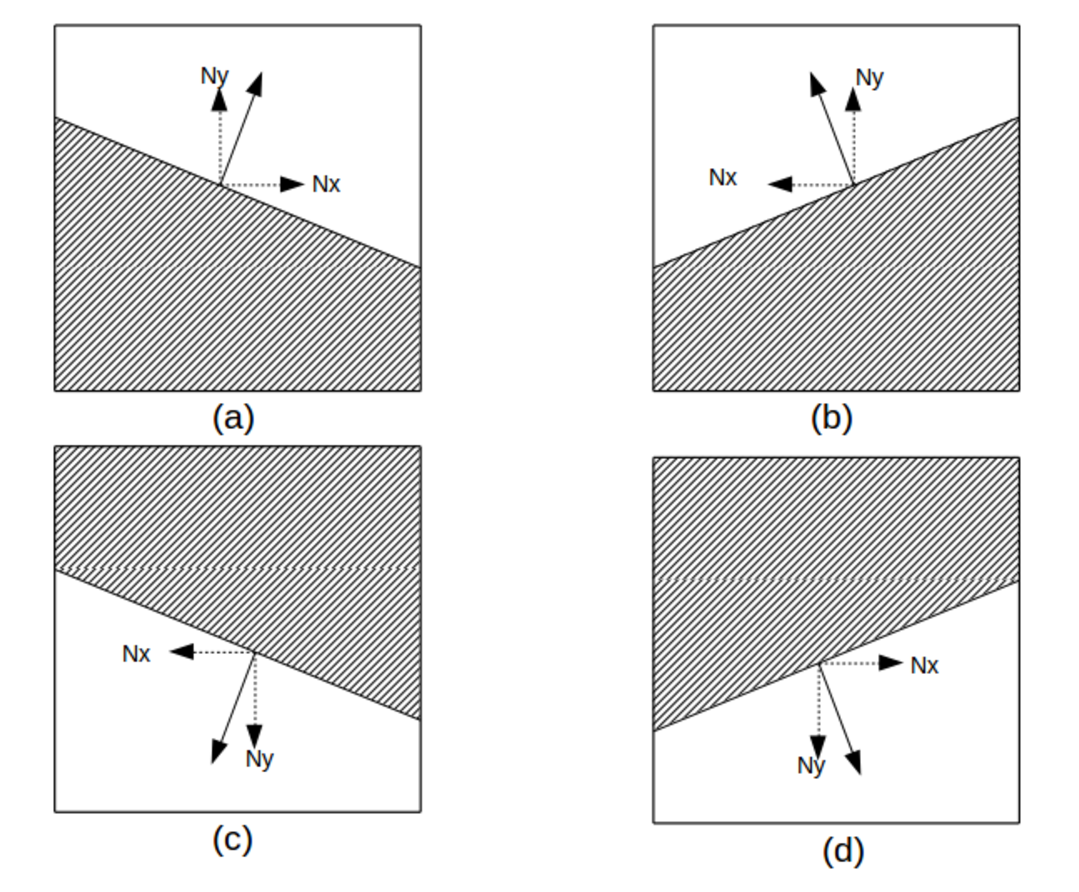
\includegraphics[scale=0.5]{quad.eps}
   \caption[Interface normal direction]{(a)First Quadrant (b) Second Quadrant (c) Third Quadrant (d) Fourth Quadrant }
  \end{figure}

\subsection{Step IV : Calculate angle, $\theta$}
 The angle, $\theta$ is the positive acute angle made by the interface with x-axis if the normal points in first and third quadrant and positive acute angle made by 
 the interface by y-axis if normal points in second and fourth quadrant. $\theta$ is defined such that if we rotate the cell such that the normal lies in first quadrant
 it should make $\theta$ with the horizontal axis. So for second and fourth quadrant the $\theta$ has to be redefined. Refer to Figure 3.2 for definition of theta. This is 
 required to do since the algorithm is developed in way it works for normal in first quadrant and all other cases has to be modified according to algorithm.
 
 \begin{figure}[H]
 \centering
  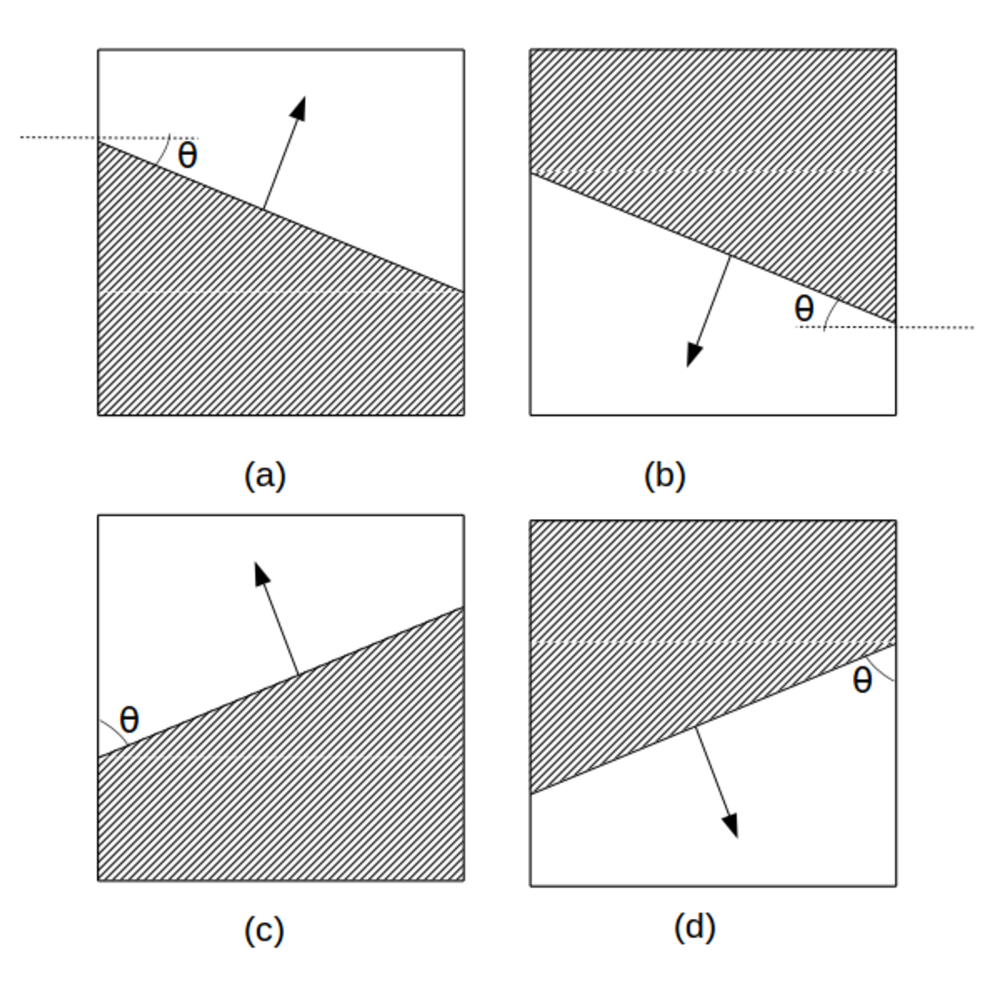
\includegraphics[scale=0.5]{angle.eps}
  \caption[Angle definition of interface]{Positive acute angle made by the interface with x-axis and y-axis}
 \end{figure}

 Equation 3.4 gives the expression for calculating $\theta$
\begin{equation}
 \theta=\frac{\pi}{2}-tan^{-1}(\frac{N_x}{N_y})
 \end{equation}

\subsubsection{Function atan() in GCC}
The function atan() in GCC returns a value between $\frac{-\pi}{2}$ and $\frac{\pi}{2}$. The slope, $\frac{N_y}{N_x}$ of normal to interface
is given as input to atan$[\frac{N_y}{N_x}$] return the value of the acute angle made by the x-axis. 
The returned value is positive when in first and third quadrant and negative when in second and fourth quadrant. 
To make it postive fabs function is used.

\begin{eqnarray}
\beta &=& atan(\frac{N_y}{N_x}) \\
\alpha &=&\lvert\beta\lvert 
\end{eqnarray}

 \begin{figure}[H]
 \centering
  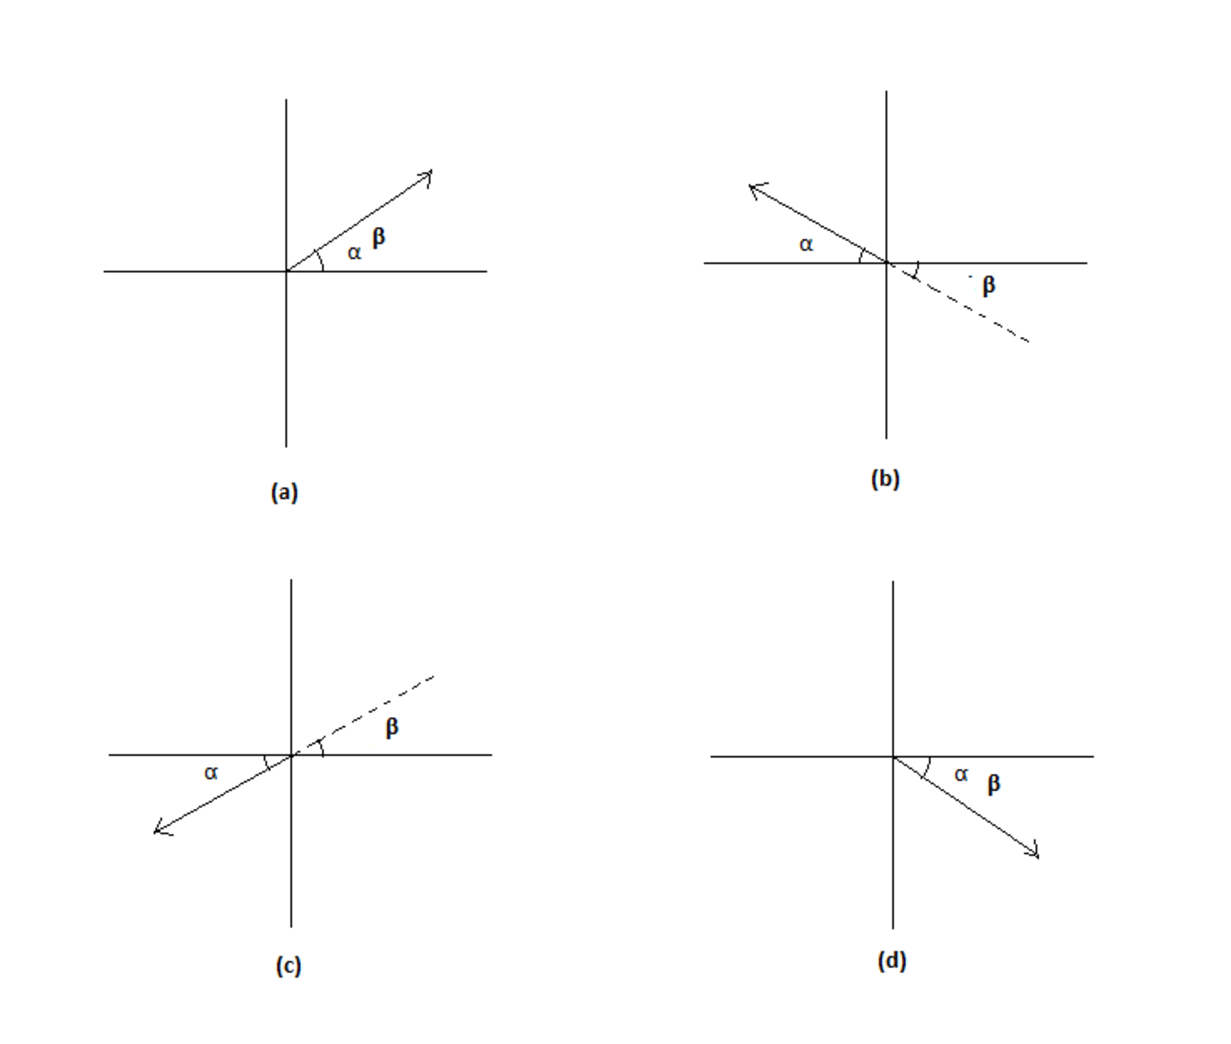
\includegraphics[scale=0.5]{atan.eps}
   \caption{Angle value returned by gcc compiler}
 \end{figure}

Hence, the expression for GCC to calculate theta becomes
\begin{equation}
 \theta=\frac{\pi}{2}-fabs(atan(\frac{N_x}{N_y}))
 \end{equation}
 Note: Every step after calculating $\theta$, will have first reorient the normal to the first quadrant.
\subsection{Step V : Identify shape}
If the volume fraction and $\theta$ is fixed then the shape of the fluid is independent of the quadrant in which the normal lies in. So there is no need to for reorientation for 
identifying shape.

From Figure 4 if the shape has to be a triangle
then,

area of fluid, $A=\Delta^2F$ \\ 

\begin{figure}[H] 
\centering
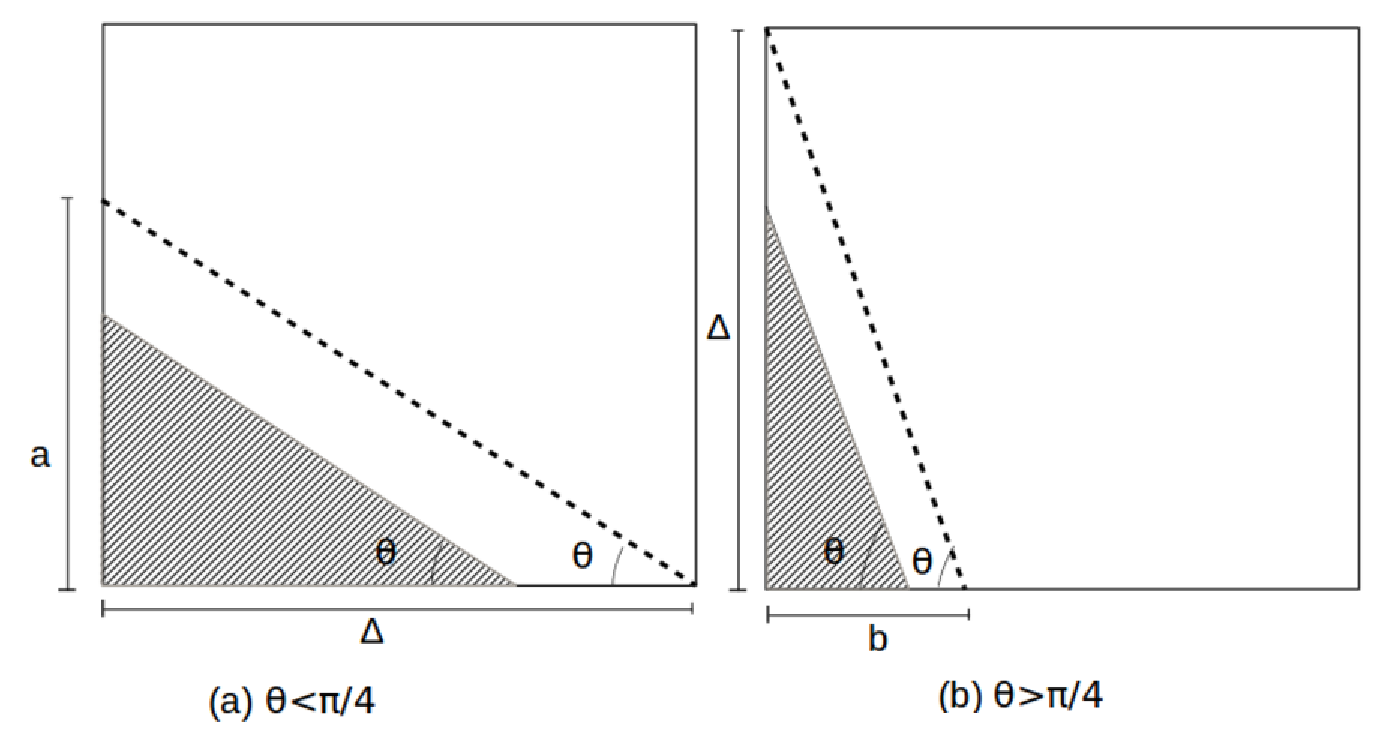
\includegraphics[scale=0.4]{triangle.eps}
\caption{Area of the triangle made by dark fluid in the cell}
\end{figure}

\begin{eqnarray}
 a&=&\Delta tan\theta \text{\quad $\theta < \frac{\pi}{4}$} \\  
 b&=&\frac{\Delta}{tan\theta} \text{\quad $\theta >= \frac{\pi}{4}$}\\
 A&<=&\begin{cases}\frac{1}{2}\Delta^2 tan\theta \text{\quad $\theta < \frac{\pi}{4}$}\\
     \frac{\Delta^2}{2tan\theta}   \text{\qquad \space $\theta>=\frac{\pi}{4}$}
    \end{cases}
\end{eqnarray}

For trapezium,
\begin{figure}[H]
\centering
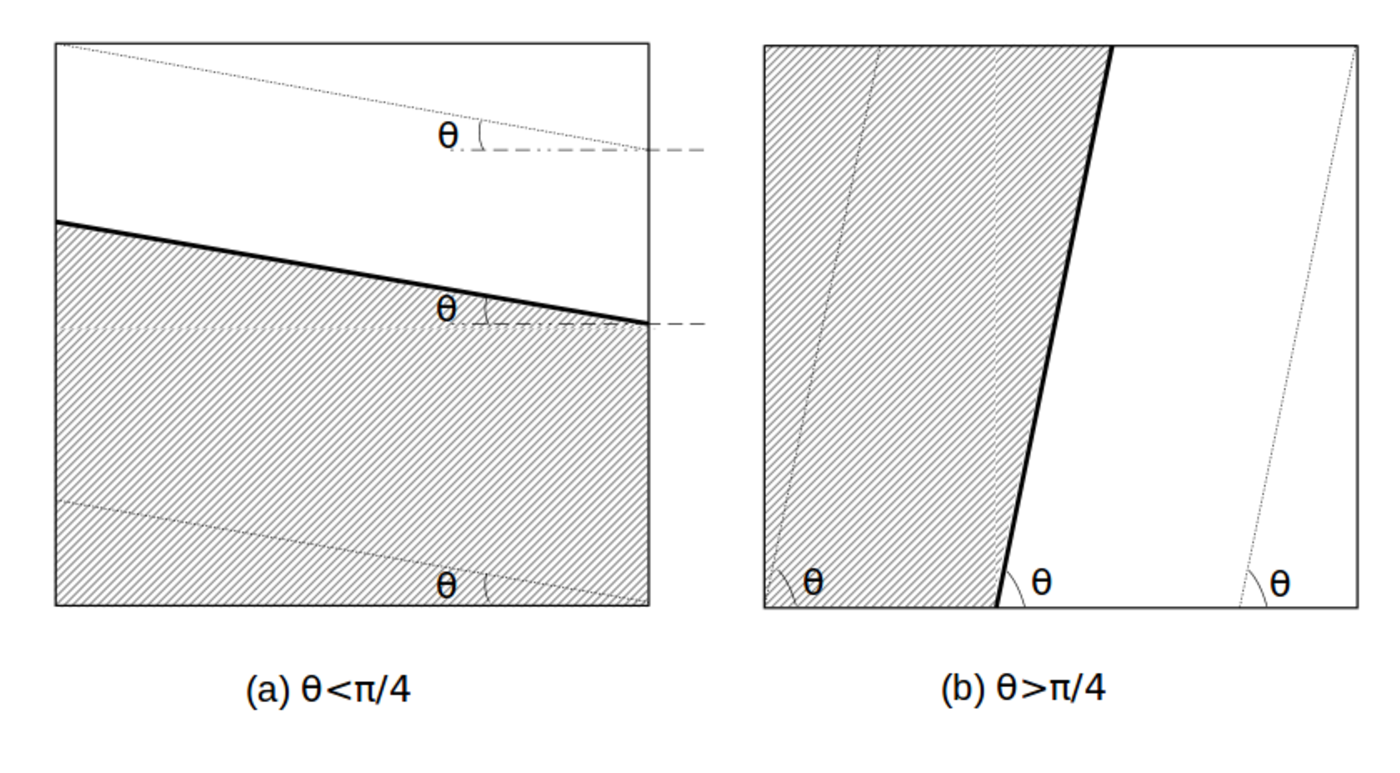
\includegraphics[scale=0.4]{trapezium.eps}
\caption{Area of a trapezium made by the dark fluid in the cell}
\end{figure}
\begin{figure}[H]
 \centering
 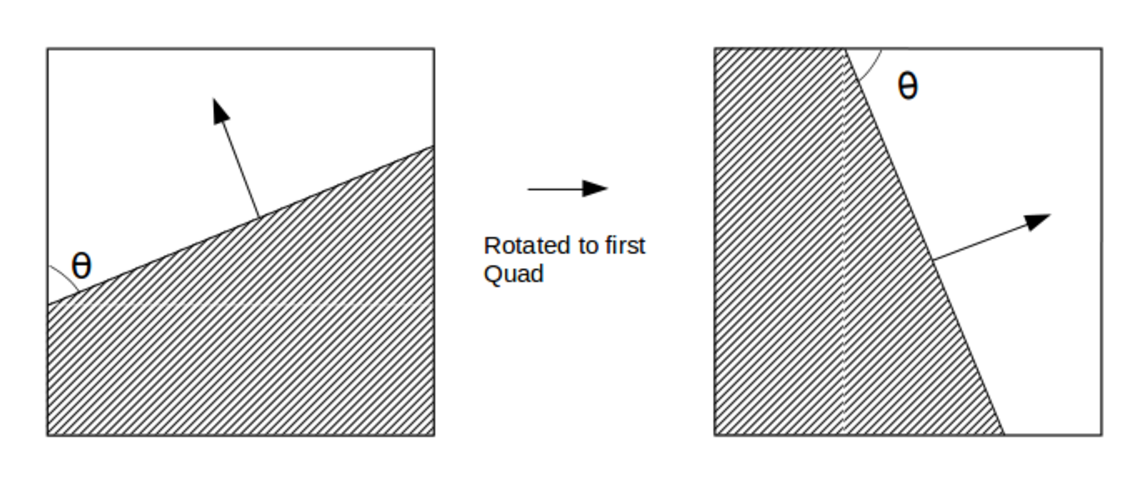
\includegraphics[scale=0.6]{2ndQuad.eps}
 \caption{When the cell is reoriented to make normal lie in first quadrant}
\end{figure}
In Figure 3.6, it can be seen that when the cell reoriented to make the normal in first quadrant the $\theta$ becomes the angle with the horizontal axis.
Hence, the same calculations can be applied to this cell for what is done for first quadrant. 
\begin{equation}
\begin{split}
 A=\begin{cases}(\frac{1}{2}\Delta^2 tan\theta,(1-\frac{1}{2}\Delta^2 tan\theta)) \quad  \theta < \frac{\pi}{4}\\
     (\frac{\Delta^2}{2tan\theta},(1-\frac{\Delta^2}{2tan\theta}))  \quad  \theta>=\frac{\pi}{4}
    \end{cases}
      \end{split}
\end{equation}
For all other cases the shape becomes a compliment of a triangle.

\subsection{Step VI : Calculate prependicular distance }
After reorientation, the prependicular distance will now be always from the LHS corner of the cell.

If shape is a triangle, then
\begin{figure}[H]
\centering
 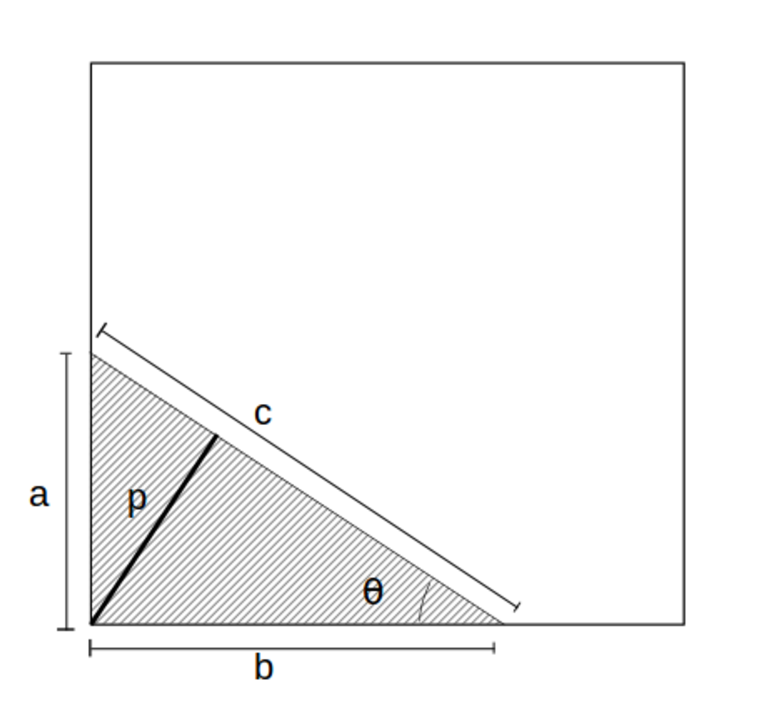
\includegraphics[scale=0.4]{triangle_p.eps}
 \caption{Prependicular distance in a triangle}
\end{figure}

\begin{eqnarray*}
c=\frac{b}{cos\theta},
\qquad b=\frac{p}{sin\theta},
\qquad  c=\frac{p}{sin\theta cos\theta},
\qquad   \frac{1}{2}pc=F\Delta^2 ,
\qquad  \frac{p^2}{sin2\theta}=F\Delta^2,
\qquad p=\sqrt{F\Delta^2sin2\theta}
  \end{eqnarray*}

If shape is a trapezium, 

  \begin{figure}[H]
  \centering
    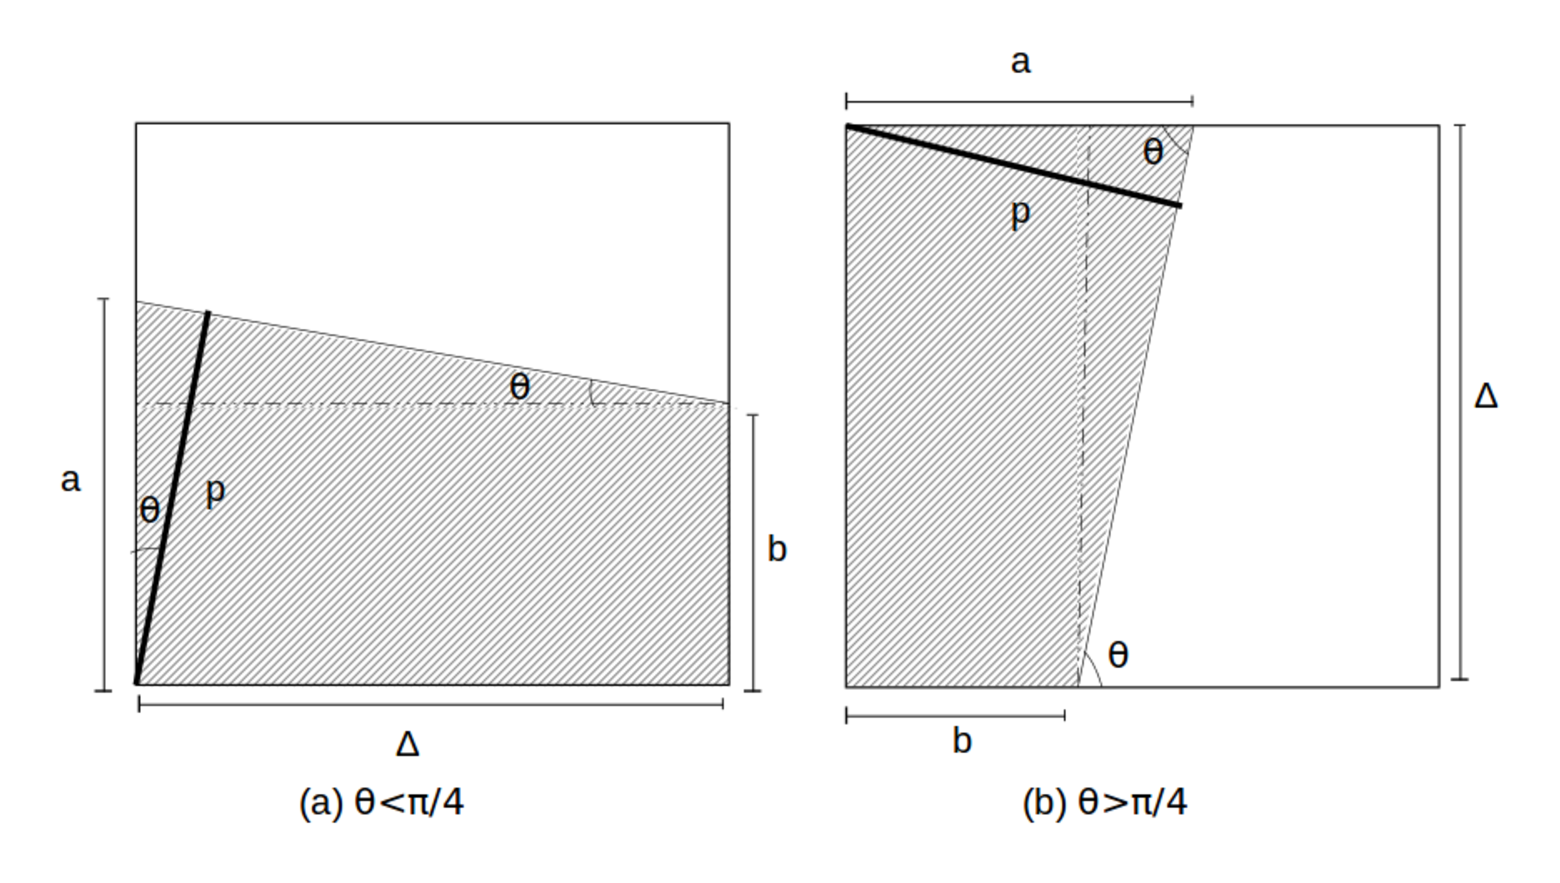
\includegraphics[scale=0.4]{trapezium_p.eps}
    \caption{Prependicular distance for a trapezium}
  \end{figure} 
  \begin{eqnarray*}
     \text{For,} \quad \theta  < \frac{\pi}{4},\\
    \qquad \Delta^2 F =\frac{(a+b)\Delta}{2},
      \qquad a=\frac{p}{cos\theta},
      \qquad tan\theta=\frac{a-b}{\Delta},
      \qquad b=\frac{p}{cos\theta}-\Delta tan\theta, \\
      \qquad \frac{1}{2}\Delta(\frac{2p}{cos\theta}-\Delta tan\theta)=\Delta^2 F,
      \qquad p=\Delta Fcos\theta+\frac{1}{2}\Delta sin\theta,
  \end{eqnarray*}
  
\begin{eqnarray*}
\
\text{For,} \quad \theta  >= \frac{\pi}{4},\\
\Delta^2 F =\frac{(a+b)\Delta}{2},
\qquad a=\frac{p}{sin\theta},
\qquad tan\theta=\frac{\Delta}{a-b},
\qquad b=\frac{p}{sin\theta}-\frac{\Delta}{tan\theta}, \\
\qquad \frac{1}{2}\Delta(\frac{2p}{sin\theta}-\frac{\Delta}{tan\theta)}=\Delta^2 F,
\qquad p=\Delta Fsin\theta+\frac{1}{2}\Delta cos\theta
\end{eqnarray*}

For compliment of triangle,
\begin{figure}[H]
\centering
 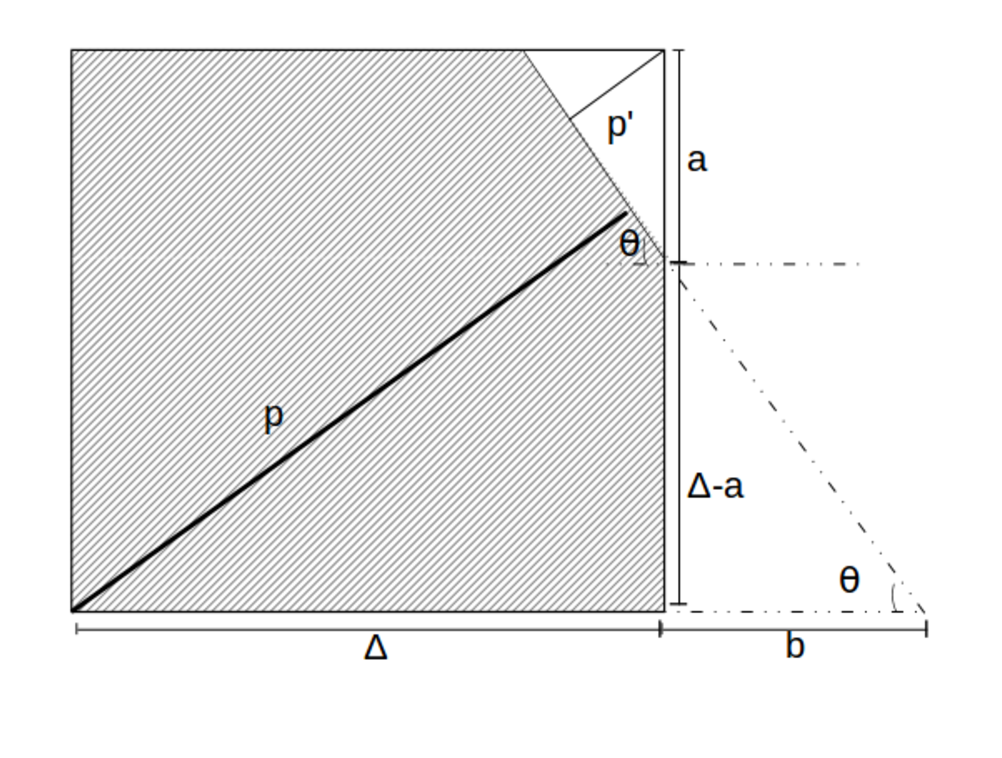
\includegraphics[scale=0.3]{compliment_p.eps}
 \caption{Prependicular distance for compliment of the triangle}
\end{figure}

\begin{eqnarray*} 
p'=\sqrt{F\Delta^2sin2\theta},
\qquad
a=\frac{p'}{cos\theta},
\qquad
b=\frac{\Delta-a}{tan\theta},
\qquad
p=\Delta(sin\theta+cos\theta)-p'
\end{eqnarray*}

\subsection{Step VII : Extrapolate line}
After, reorientation of the line to the first quadrant. A line can be constructed with $\theta$ and prependicular distance using normal form,
\begin{figure}[H]
 \centering
 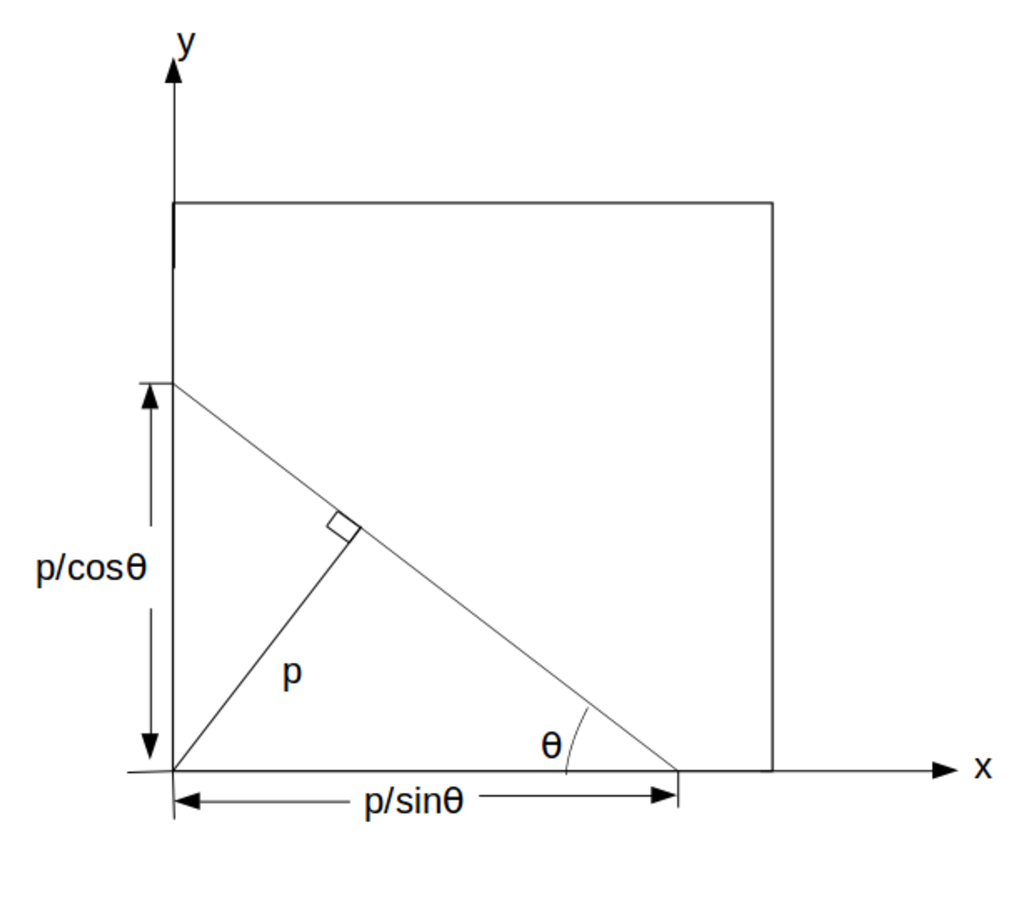
\includegraphics[scale=0.4]{normal_form.eps}
 \caption{Normal form of a line in the cell}
\end{figure}
\begin{equation}
 x\sin\theta+y\cos\theta = p
\end{equation}

Refer to Figure 3.10 for extrapolation,

\begin{figure}[H]
 \centering
 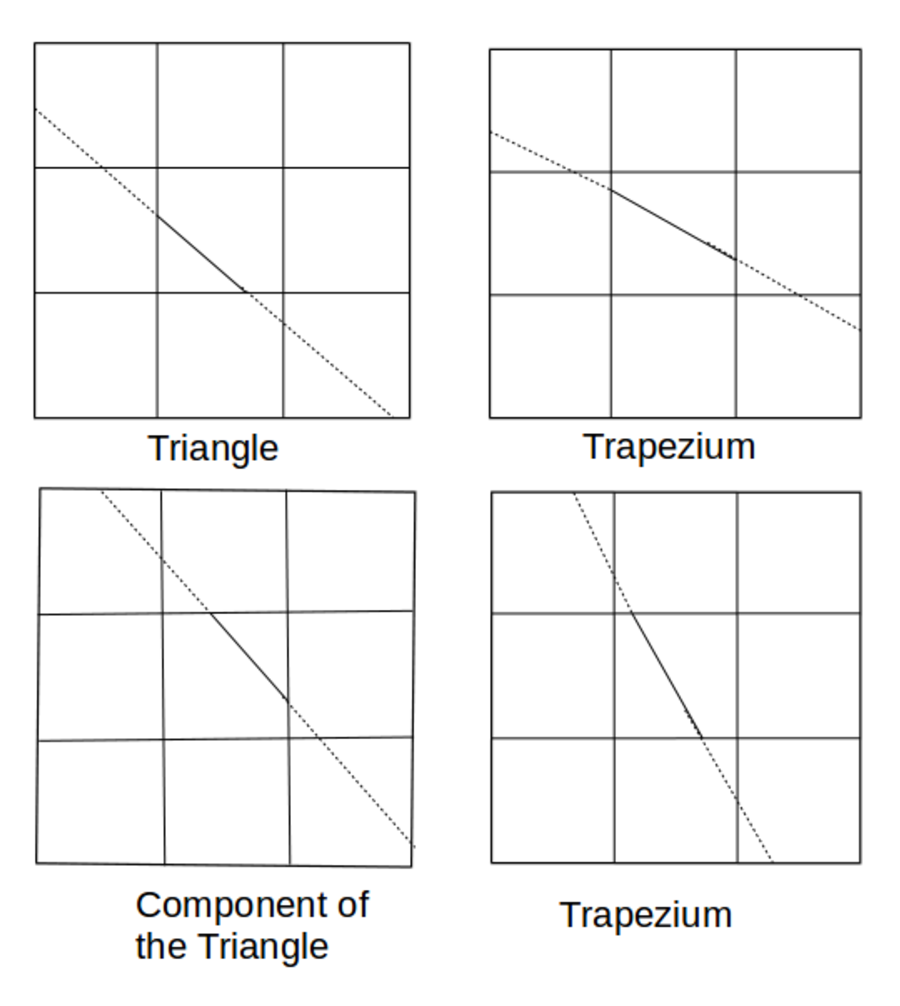
\includegraphics[scale=0.4]{extrapolate.eps}
 \caption{Extrapolation of the line in 3 X 3 cell}
\end{figure}

After extrapolation the new volume fraction calculated under each cell below the line, which then used to calculate the norm.
\subsection{Step VIII: Calculate Norm}
Let the new volume fraction calculated be $\widetilde F_{r,c}$. Now the norm which is here the difference of original volume fraction and new 
volume fraction calcuated after the extrapolation are squared and then summed over 3 X 3 stencil. Also, called as $L^2$ norm, \\
\begin{equation}
 L^2(\widetilde F) =  \sum_{k,l=-1}^{1}(\widetilde F_{r+k,c+l}-F_{r+k,c+l})^2
\end{equation}

\subsection{Step IX : Minimize Norm}
After calculating norm the initial guess of slope and $\theta$ is changed with small step size but it should not be confused with rotation of interface or normal.
All the steps are repeated to after modifiying theta and norm is again calcuated. This process repeats when a minima of norm reached. And the final values of $\theta$,
shape, and quadrant are assigned to the cell.

\section{Advection}
The equation 3.1 is also solved using geometrical technique by calculating fluxes across the cells and then updating the F-field in each time step. The direct finite differencing
will lose the discontinuos property of F-field and cause smearing of interface.
The flux is calculated through the wall of the cells in X an Y directions.

For first quadrant all cases are discussed below, \\
Note:- for all other quadrants the algorithm passes the values as if the normal is in first quadrant and the values returned by it are passed accordingly to 
the structure. The interface angle with horizontal axis (after rotating the normal to first quadrant)$\theta$ is calculated and stored in the structure.

For X-Flux when velocity in x-direction, u is positive then only the right wall of the left cell will affect the flux (See Figure 11)
\subsection{Flux Calculation}
\subsubsection{Triangle}
For a triangle there are two cases:-\\
if $\Delta-udt>x_0$, Nothing will leave from the right wall \\
if $\Delta-udt<x_0$, A triangle leaves. \\
where $x_0$ is the x at $y=0$.
\begin{figure}[H]
 \centering
 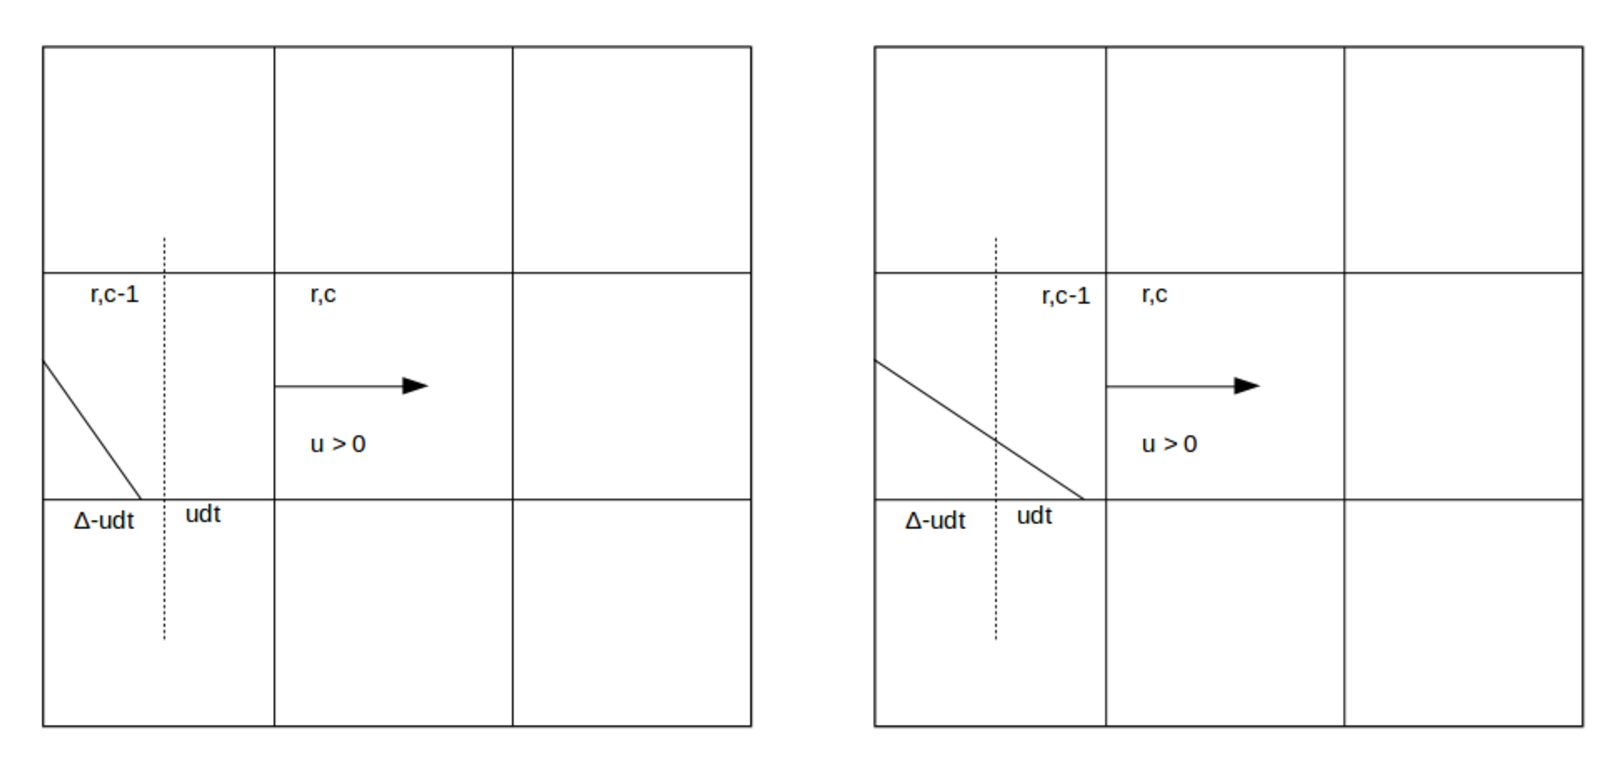
\includegraphics[scale=0.4]{ad_triangle.eps}
 \caption{Cases for a triangle in flux calculation}
\end{figure}
For the second case where a part of triangle leaves which is also a triangle, \\
the area of the part which leaves is given by,
\begin{equation*}
 Flux = \frac{1}{2}(x_0 - del + udt)^2 tan\theta
\end{equation*}

\subsubsection{Trapezium}
Two types of trapezium can be in the first quadrant, $\theta<\frac{\pi}{4}$, and $\theta>\frac{\pi}{4}$, \\
(See Figure 12 and 13) \\
\begin{figure}[H]
\centering
 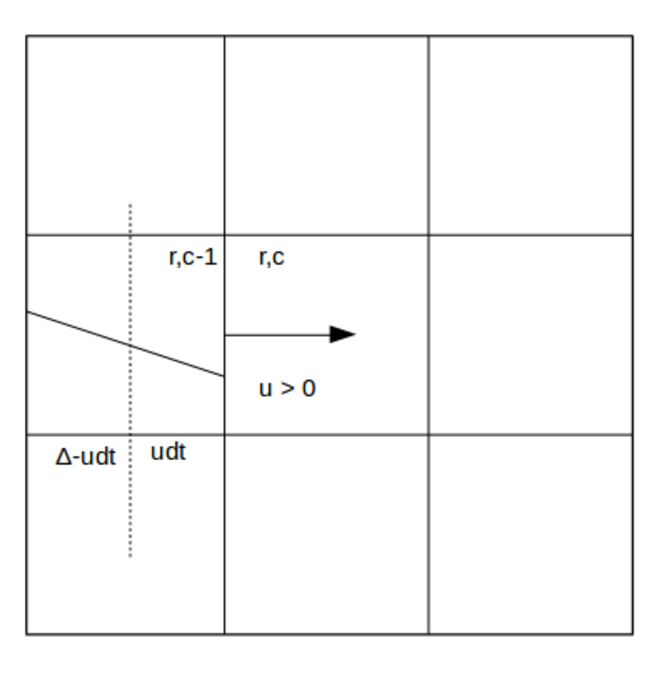
\includegraphics[scale=0.4]{ad_trapezium.eps}
 \caption{Flux calculation for trapezium for $\theta<\frac{\pi}{4}$}
\end{figure}
For $\theta<\frac{\pi}{4}$,
\begin{eqnarray*}
 Flux = \frac{1}{2}( y_0 - ((\Delta - udt)*tan\theta) + y_del )*udt \\
\end{eqnarray*}

For $\theta>\frac{\pi}{4}$, \\
\begin{figure}[H]
 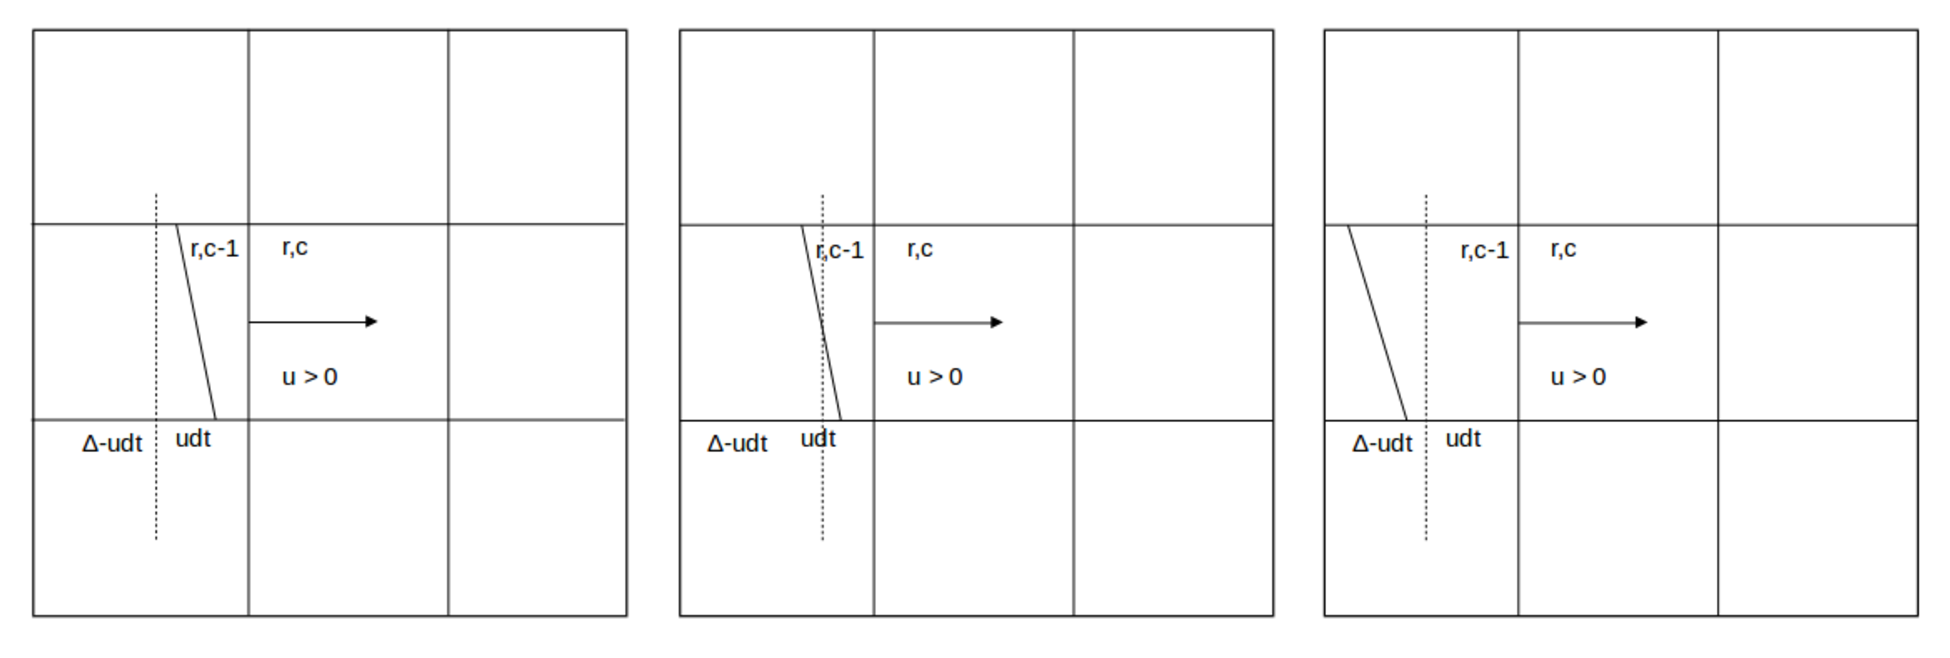
\includegraphics[scale=0.4]{ad_trap_pi4.eps}
 \caption[Different cases for flux calculation for trapezium]{(a)$\Delta-udt<x_{del}$, (b)$\Delta-udt>=x_{del}$ and $\Delta-udt<x_0$, (c)$\Delta-udt>=x_0$}
\end{figure}

For $\Delta-udt<x_{del}$, a trapezium leaves the cell and the Flux is given by,

Flux = $\frac{\Delta}{2}(x_{del} - (2(\Delta - udt)) + x_0)$\\

For $\Delta-udt>=x_{del}$ and $\Delta-udt<x_0$, a triangle leaves the cell and the flux is given by, \\
Flux =$\frac{1}{2\tan\theta} (y_0 - (\Delta - udt)tan\theta))^2$ \\

For $\Delta-udt>=x_0$, nothing leaves from the cell \\

\subsubsection{Compliment of a triangle}
For compliment of a triangle two cases arise, (See Figure 15)
\begin{figure}[H]
 \centering
 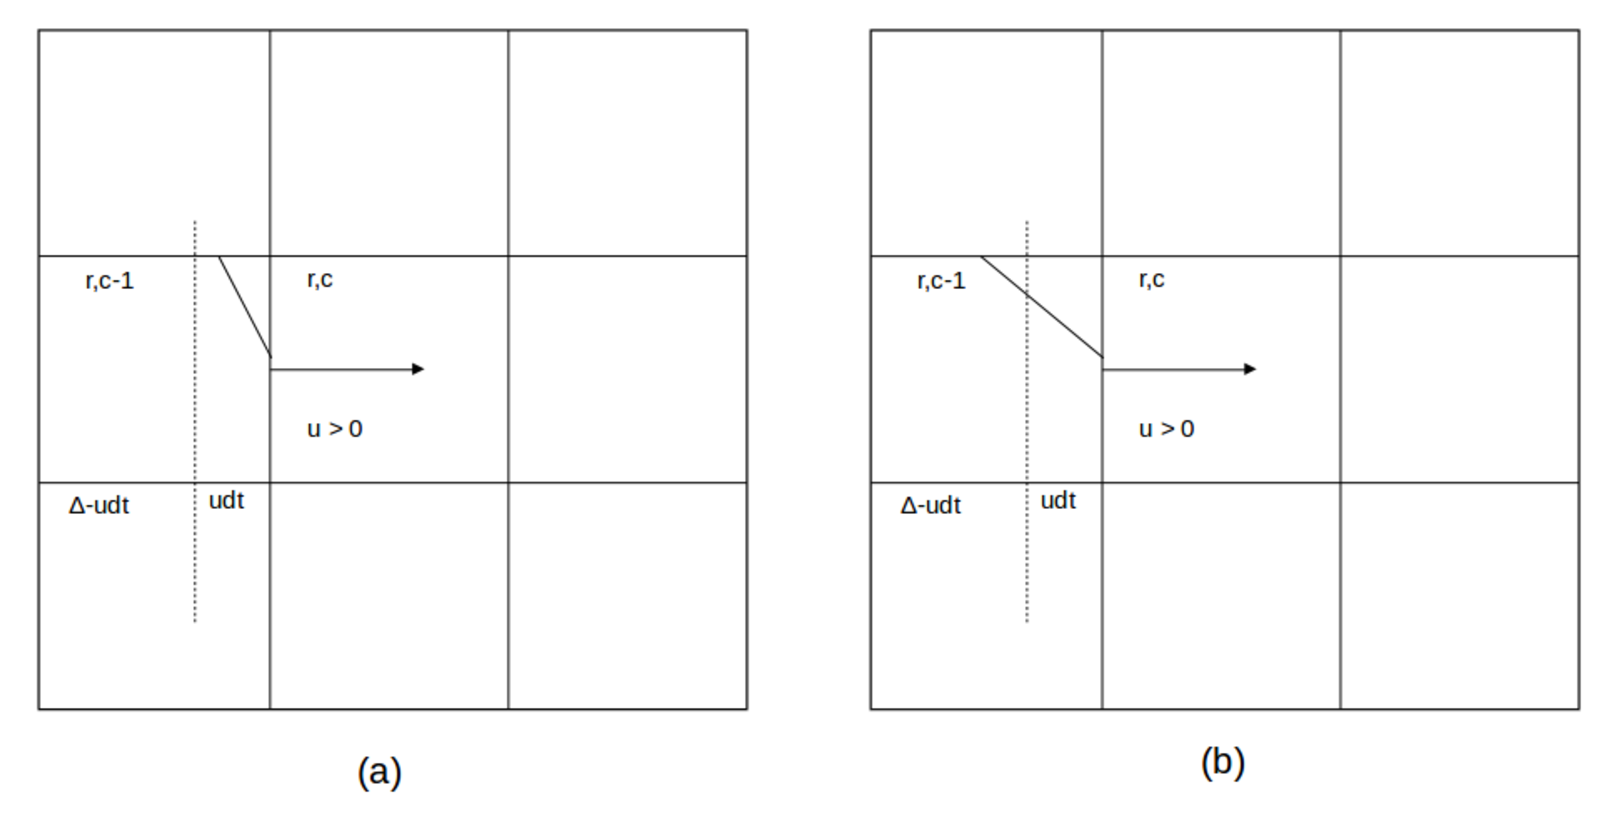
\includegraphics[scale=0.4]{ad_comp.eps}
 \caption[Different cases for flux calculation for compliment of a triangle]{(a)$\Delta -udt < x_{del}$, (b)$\Delta -udt >= x_{del}$}
\end{figure}

if $\Delta -udt < x_{del}$, A 5-Sided figure leaves,  and Flux is given by, \\
$Flux = \Delta(x_{del} - \Delta + udt)) + \frac{1}{2}((\Delta + y_{del})(\Delta - x_{del}))$,  (sum of rectangle and trapezium) \\

or, if $\Delta -udt >= x_{del}$, A trapezium leaves, and Flux is given by, \\
Flux =  $\frac{udt}{2}( y_{del} + y_0 - (\Delta - udt)\tan\theta)$

  
\subsection{Rectangle}
For rectangle (See Figure 17 )
\begin{figure}[H]
 \centering
 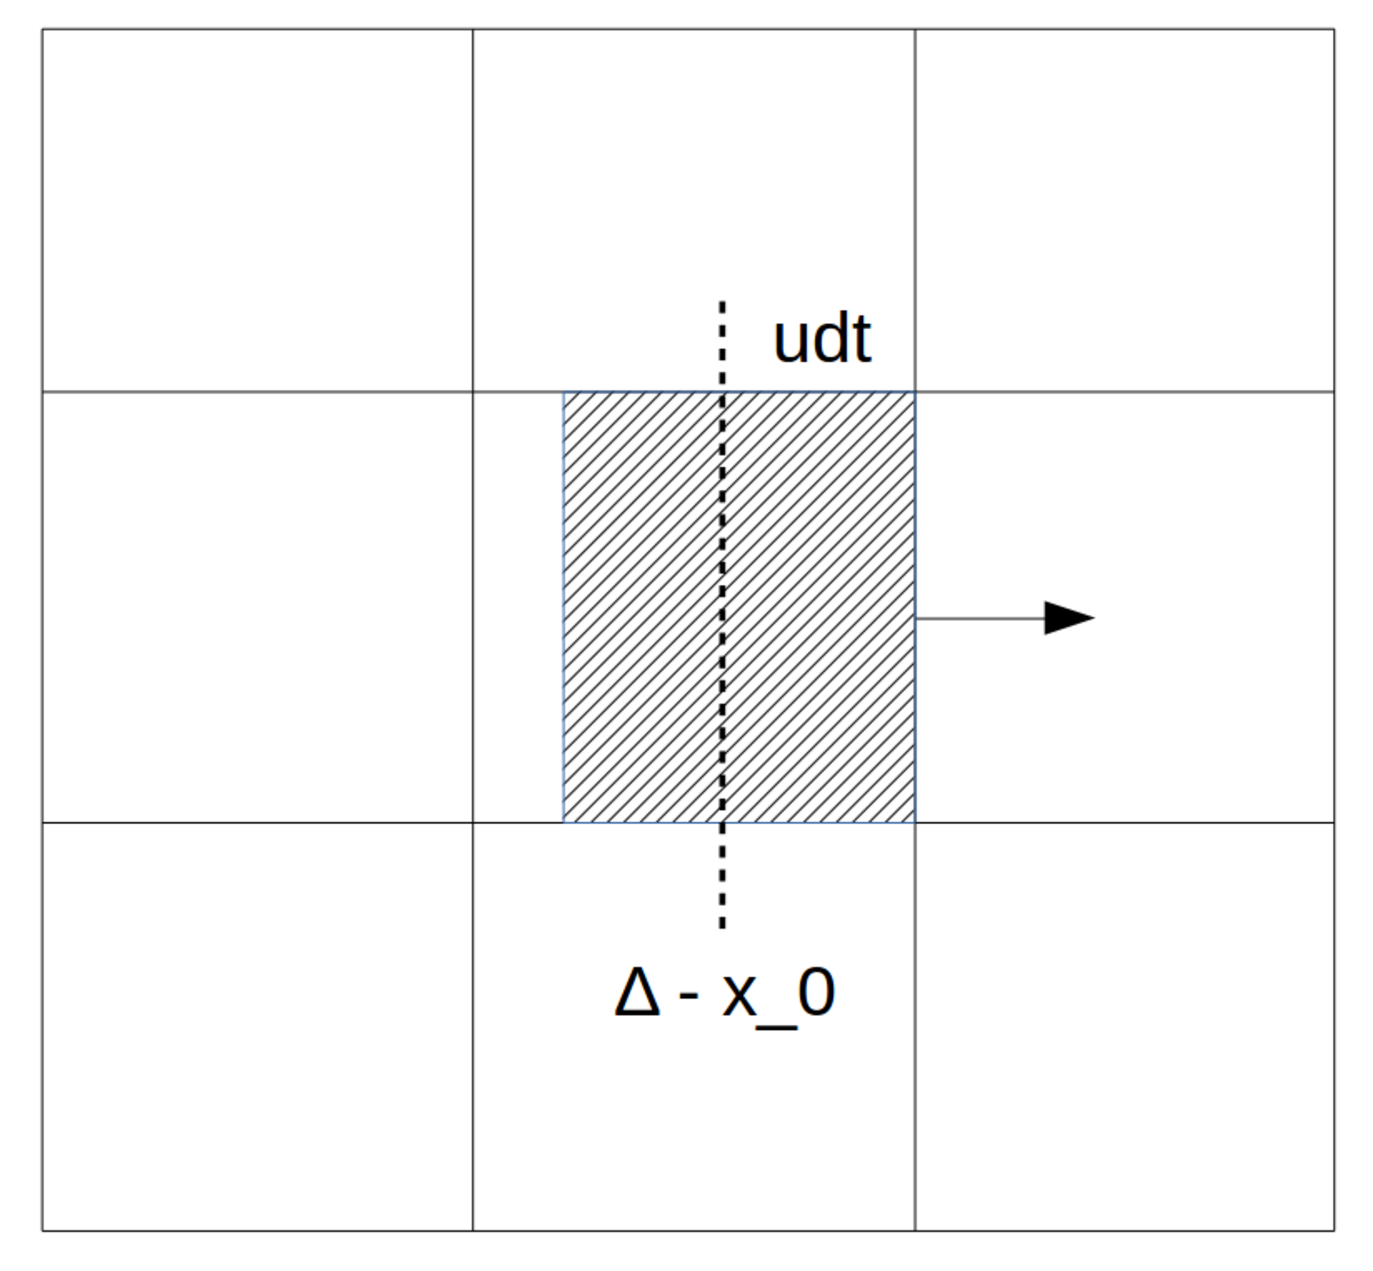
\includegraphics[scale=0.2]{ad_rect.eps}
 \caption{Flux calculation for rectangle}
\end{figure}

if $\Delta -udt <= x_{0}$, A Nothing leaves \\
$Flux = 0$

or, if $\Delta -udt >= x_{0}$, A rectangle leaves, and Flux is given by, \\
$Flux =  \Delta(udt)$


